% This is based on the LLNCS.DEM the demonstration file of
% the LaTeX macro package from Springer-Verlag
% for Lecture Notes in Computer Science,
% version 2.4 for LaTeX2e as of 16. April 2010
%
% See http://www.springer.com/computer/lncs/lncs+authors?SGWID=0-40209-0-0-0
% for the full guidelines.
%

\documentclass{llncs}
\usepackage{graphicx}
\usepackage[usenames, dvipsnames]{color}

\begin{document}

\title{Our Project}
%
\titlerunning{our project}  % abbreviated title (for running head)
%                                     also used for the TOC unless
%                                     \toctitle is used
%
\author{Tor Dj\"{a}rv\inst{1} \and Noam Gavrielov\inst{2}\and Luca Riz\inst{3}}
%
\authorrunning{Tor Dj\"{a}rv et al.} % abbreviated author list (for running head)
%
%%%% list of authors for the TOC (use if author list has to be modified)
\tocauthor{Tor Dj\"{a}rv, Noam Gavrielov, and Luca Riz}
%
\institute{University of \dots\\
\and
University of \dots
\and
Department of Physics, University of Trento, Via Sommarive 14, I-38123 Trento,
Italy}

\maketitle              % typeset the title of the contribution

\begin{abstract}
\dots
\keywords{computational geometry, graph theory, Hamilton cycles}
\end{abstract}
%
\section{NushellX}
%
%
In this part we present the results we obtained using NushellX \cite{nush} and we comment on them. We focus  on the sd-shell, specifically on oxygen isotopes and their properties. In the first subsection we analyze the spectra of oxygen isotopes and the capability of different interactions (i.e. new-usd family of interactions \cite{usd} (usda and usdb) and couple cluster effective interaction \cite{ccei} (ccei)) to reproduce spectra. The second subsection is devoted to the study of Fermi and Gamow-Teller $\beta$-decay of $^{22}$O and how usdb and ccei interactions fulfill sum rules.

\subsection{Oxygen isotopes spectra with different interactions}
%
In order to see how the different interactions describe the oxygen isotopes we decided first to analyze how different interaction reproduce the excitation energy of the first $2+$ state in even-even oxygen isotopes from $^{18}$O to $^{26}$O and compared it with experimental. This gives also an overlook on where the shell closure is, since when the excitation energy from g.s. to the first excited $2+$ state (in even-even nuclei) is maximum indicates that we are in a shell closure configuration.

\begin{figure}[htb!]
\centering
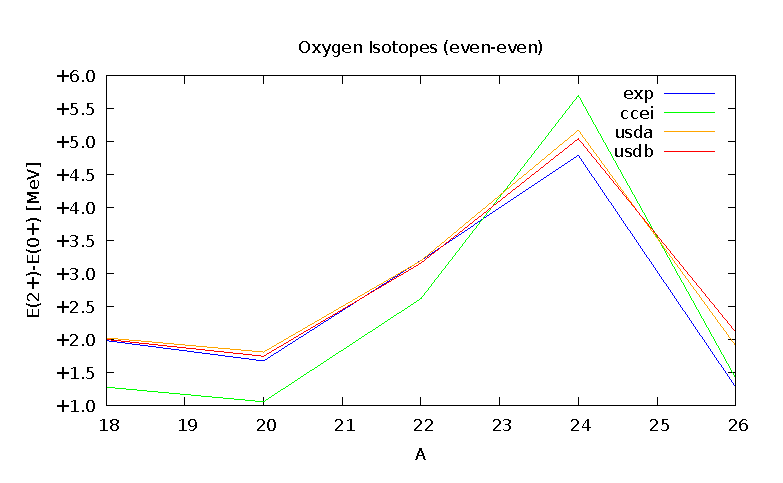
\includegraphics[width=0.8\textwidth]{2+_over_0+.eps}
\caption{Excitation energy of the first $2+$ state in oxygen isotopes (even-even).}
\label{fig:2+/0+}
\end{figure}

As expected usda and usdb interactions give pretty similar results and are in good agreement with experimental results. Both usda and usdb interaction give a good description of the shell closure at $^{24}$O. Since usdb has more linear combination of parameters than usda interactions we should expect a better agreement with experimental results and indeed it is what we obtained as shown in Figure \ref{fig:2+/0+}. The ccei interaction underestimates the excitation energies up to $^{26}$ oxygen, while at shell closure it emphasize this effect overestimating the first $2+$ state energy. It is interesting to note that ccei interactions seems to give a good description in really-reach neutron isotopes, close to the neutron drip line.

We also explored the spectra of even-odd oxygen isotopes. Since we wanted to compare it with an isotope where many experimental data are available we choose to analyze the spectrum of $^{19}$O as show in Figure \ref{fig:19O}. 
\begin{figure}[htb!]
\centering
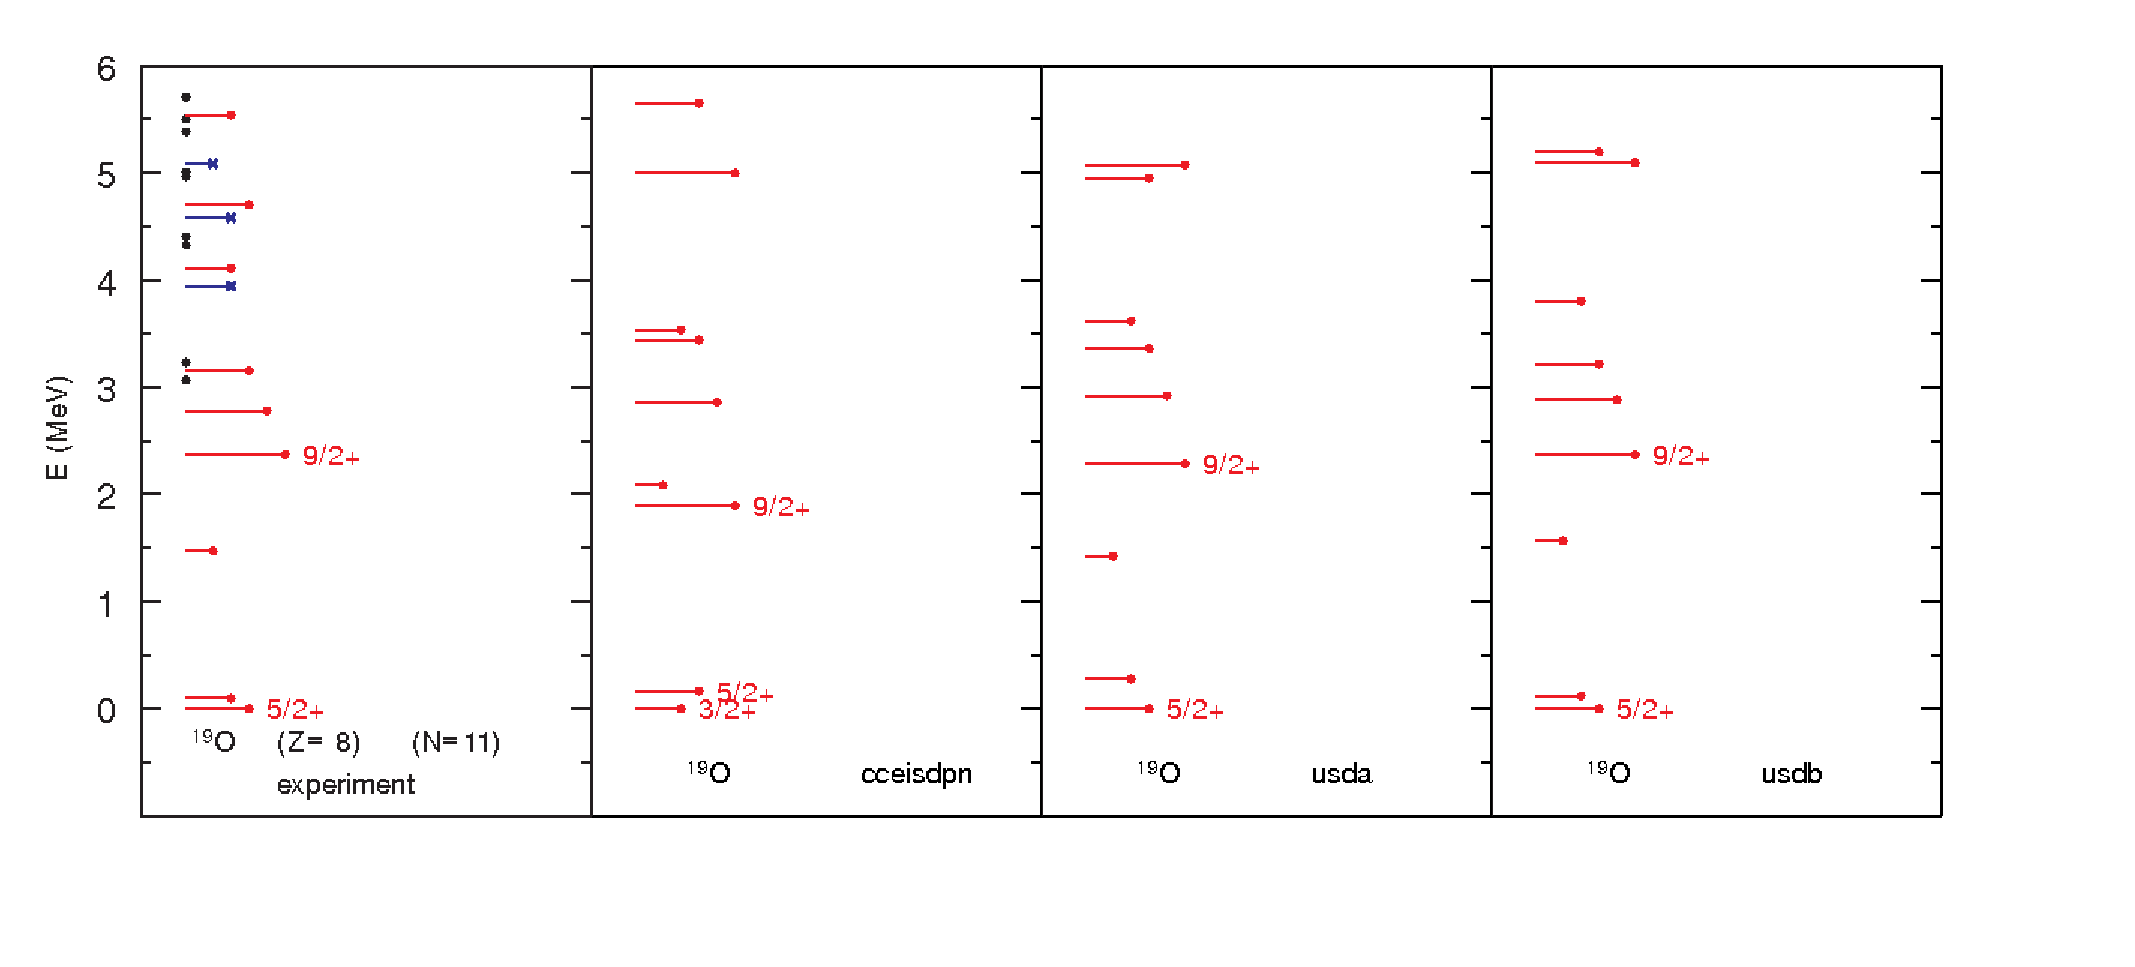
\includegraphics[width=\textwidth]{19O.eps}
\caption{$^{19}$O spectrum with different interactions compared to experiments.}
\label{fig:19O}
\end{figure}
At first look it is clear that usda and usdb reproduce the spin of the ground state while the ccei exchanges the energy levels of the first excited $3/2+$ and the gs. This could be reasonable since if we look at the experimental spectrum the ground state and the first excited state are really close by. To look even more in detail the difference between usdb and usda, the usdb interaction is really capable to reproduce the experimental results even at higher excitation energies. Note that the experimental results show also negative parity states (blue states), which are not included in our theoretical calculations since we are working in the sd model space, which can  describe only positive parity states. For completeness black dots in the experimental panel indicates states which have not been assigned to a definite parity.
%
\subsection{\textcolor{red}{(Spectroscopic Factors?)}}
\textcolor{red}{Not sure if we add also the part on spectroscopic factors \dots I think if I add also this part it becomes too long.}
%

%
\subsection{Fermi and Gamow-Teller $\beta$-decay of $^{22}$O.}
%
The bounty of an interaction is not simply to be able to describe energy spectra of different isotopes, but we need to look at different observables. We decided to analyze the $\beta$-decay of $^{22}$O to $^{22}$F.
We perform the calculations using NushellX both for the usdb and ccei interactions. 
\begin{table}[h!]
\caption{Sum Rules}
\begin{center}
\begin{tabular}{l@{\qquad}l@{\qquad}r@{\qquad}rl}
\hline
\multicolumn{1}{l}{\rule{0pt}{12pt}
                   }&\multicolumn{1}{l}{\rule{0pt}{12pt} sum rule}&\multicolumn{1}{l}{ccei}&\multicolumn{2}{l}{usdb}\\[2pt]
\hline\rule{0pt}{12pt}
sum b(f)            &  $N_i-Z_i=6$   & 5.9993 & 6.0000 &\\
sum qf$\cdot$b(gt)  &  $\ge 3\cdot(N_i-Z_i)=18$  & 6.0346 & 10.0335 &\\[2pt]
\hline
\end{tabular}
\end{center}
\end{table}

It is interesting to point out that both interactions fulfill the theoretical Fermi sum rule, but in different ways.
With ccei interaction the contribution to Fermi sum rule b(f) splits among different states: this is because with this effective interaction we have a mixing between closed lying levels, while the usdb interaction gives all the contribution to b(f) in one single state, which is the isobar analogue of the $^{22}$O \textcolor{red}{(is this true? - Ch. 44 Brown's notes)}. 
\textcolor{red}{(Anyone has more to say about Gamow-Teller sum rule?)}

Let us compare the results obtained with the two different interactions to the experimental results for the q-value and the half-time life. Note that one has to include more than only the default ten levels for each spin state in NushellX in order to get significant results, otherwise too much information is neglected.
\begin{table}[h!]
\caption{q-value and t$_{1/2}$}
\begin{center}
\begin{tabular}{r@{\qquad}r@{\qquad}r@{\qquad}r@{\qquad}l}
\hline
\multicolumn{1}{l}{\rule{0pt}{12pt}
                   }&\multicolumn{1}{l}{exp}&\multicolumn{1}{l}{ccei}&\multicolumn{2}{l}{usdb}\\[2pt]
\hline\rule{0pt}{12pt}
q-value [MeV]   &     6.489 & 6.847 & 8.437 &\\
t$_{1/2}$ [sec] &     2.25  & 0.478 & 2.620 &\\[2pt]
\hline
\end{tabular}
\end{center}
\end{table}

The results we get are pretty interesting compared with experiments. The ccei interaction gives a really good description of the q-value, but underestimates the half-lifetime, while the usdb interaction is in good agreement with the experimental value for the half-lifetime, but slightly overestimates the q-value.

%
\paragraph{Notes and Comments.}
\textcolor{red}{I think we should make the conclusions together.}

%
% ---- Bibliography ----
%
\begin{thebibliography}{3}
%
\bibitem {nush}
B. A. Brown and W. D. M. Rae, Nuclear Data Sheets 120, 115 (2014)
\bibitem {usd}
B. A. Brown and W. A. Richter, Physical Review C 74, 034315 (2006)
\bibitem {ccei}
G. R. Jansen, M. D. Schuster, A. Signoracci, G. Hagen and P. Navr\'atil, Physical Review C 94, 011301(R) (2016)

\end{thebibliography}

\end{document}
